\documentclass{trchesh}
\usepackage{trmath}
\usepackage{trsym} 

\usepackage{cmbright}
\setlayout[page-orient=landscape, size=10]{hardcopy}
\makeatletter
\def\note{\ifexpmode{\@gobble}{\endnote}}
\makeatother

\hypersetup{
  pdftitle={Шпора по электроду},
  pdfauthor={taxus},
  pdfsubject={Электродинамика},
  pdfkeywords={Электродинамика;СПбГУ;by-taxus}
}
\columnseprule=0.1dd
\def\arraystretch{1.3}
\setlist[enumerate,1]{leftmargin=1.6em}
\setlist[itemize,1]{leftmargin=2em, label=$\triangleright$}

\def\waveop{\mathop{\boldsymbol\Box}}

\newcommand{\deflabel}[1]{
  \makebox[\labelwidth][l]{%
    \parbox[t]{\labelwidth}{\hspace{0pt}\textsf{#1}}%
  }~::
}
\newenvironment{defs}[1][\hspace{12ex}]%
  {\begin{list}{}{%
        \let \makelabel=\deflabel%
        \setlength{\labelwidth}{\widthof{#1}} %
        \setlength{\leftmargin}{\labelwidth+\labelsep}%
        \itemsep=0pt %
      }}%
  {\end{list}}
\newenvironment{facts}{\begin{list}{$\triangleright$}{}}{\end{list}}

\graphicspath{{img/}}
\begin{document}
\begin{multicols*}{3}\raggedright
\parindent=0pt
\paragraph{Уравнения Максвелла}
\begin{enumerate}
  \item Теорема Гаусса: $\oint \v E \cdot \del \v s = 4 \pi Q$.
  \item Закон Фарадея: $\oint\v E \cdot \del \v l = - \frac{1}{c} \pder{\Phi}{t}$, \\
    $\Phi=\int \v B \cdot \del \v s$
  \item Закон Био-Савара-Лапласа: $\v B = \frac{1}{c} \, \frac{\v j \times \v R}{R^3}$
  \item $\oint \v B \cdot \del \v s = 0$
  \item Закон Ампера: $\oint \v B \cdot \del \v l = \frac{4 \pi}{c} \int \v j \cdot \del \v s$
  \item Уравнение неразрывности: $\pder \rho t  + \div \v j = 0 $
  \item Сами уравения Максвелла: \par\vspace{1ex}$
    \begin{aligned}
      &\div \v E &&=&& 4 \pi \rho \\
      &\div \v B &&=&& 0 \\
      &\rot \v E &&=&& - \frac 1 c \, \pder{\v B}{t} \\
      &\rot \v B &&=&& \frac 1 c\, \pder{\v E}{t} + \frac{4 \pi}{c}\v j
    \end{aligned}$
\end{enumerate}

\paragraph{В среде}
\begin{enumerate}
  \item Поляризация и намагниченность \\
    $\begin{aligned}
    \v P \that\v j_{\mathrm{pol}} &=\pder{\v P}t,\;\rho_{\mathrm{pol}} =-\div \v P,\\
    \v M \that \v j_{\mathrm{m}} &= c \rot \v M \\
    \{\rho, \v j\}_{\mathrm{int}} &= \{\rho, \v j\}_{\mathrm{pol}} + \{\rho, \v j\}_{\mathrm{m}}
    \end{aligned}$
\item В сильнопеременных  \par
$
\begin{aligned}
  \rho_{\mathrm{int}} &= - \div \v P \\
  \v j_{\mathrm{int}} &= \pder{\v P}{t}  + c \rot \v M
\end{aligned}
$
\item $\v D = \v E + 4 \pi \v P$, $\v H = \v B - 4 \pi \v M$
\item Уравнения Максвелла в среде: \par
  $ \begin{aligned}
        \div \v D &= 4 \pi \rho_{ex} \\
        \rot \v H &= \frac 1 c \, \pder {\v D} t + \frac{4\pi}{c} \,
        (\v j_{ex} + \v j _{c})           
      \end{aligned}$
\item Материальные уравнения (простейшие)\par
  $\v D = \varepsilon \v E,\;\v B = \mu \v H ,\;\v j_c = \sigma \v E$
\item Дисперсия, варианты \par
  $ \begin{aligned}
    \v D (\v r,t) &= \int_{-\infty}^t f (t' - t, \v r)\,\v E(\v r, t')\, \del t \\
    \v D (\v r,t) &= \int_{\Delta V} g(\v r' -\v r, t)\,\v E(\v r, t')\, \del V
  \end{aligned} $ \par
$f,g$~--- функция отклика.
\end{enumerate}


\paragraph{Энергетические соотношения}
$
  \begin{aligned}
    w &= \frac{1}{8 \pi} \, (\varepsilon E^2 + \mu H^2) \\
    \v S &= \frac{c}{4 \pi} \, \v E \times \v H \\
    \pder{w}{t} + \div \v S &= - \sigma E^2 - \v E \cdot \v j_{ex}
  \end{aligned}
$ \par
Так что если внешние силы не совершают работы, 
энергия лишь убывает (за счёт выделения тепла).

\paragraph{Потенциал}
\begin{enumerate}
  \item Вид потенциала:
    $ \v E = - \frac 1 c \pder{\v A} t  - \nabla \varphi$,
    $\v B = \rot \v A$
  \item Калибровочная инвариантность:
    $ \left\{\begin{aligned}
      \v A' &= \v A - \nabla \chi \\
      \varphi' &= \varphi + \frac{1}{c} \, \pder{\chi}{t}
  \end{aligned}\right.$
  \item Калибровка  Лоренца: 
      $\frac{\varepsilon \mu}{c} \, \pder{\varphi}t + \div \v A = 0$%
      \note{при этом подходят все $\chi \that \waveop \chi = 0$}
    \item Уравнения Максвелла примут вид: 
      $
      \begin{aligned}
        \waveop \varphi &= \frac{4 \pi}{\varepsilon}\, \rho, \\
        \waveop \v A &= \frac{4 \pi \mu}{c} \, \v j, 
        \text{ где }\waveop = \frac{1}{v^2} \, \pder[2]{}{t} - \nabla,
        v = \frac{c}{\sqrt{\varepsilon \mu}} 
      \end{aligned}
      $
\end{enumerate}
\paragraph{Волновые уравнения}
$
\begin{aligned}
\waveop \v E = 0, \; \waveop \v B  =0 \\
\waveop \v A =0, \; \waveop \varphi  =0  \qquad (\waveop \chi = 0 )
\end{aligned}
$

Ещё можно $\varphi$ занулить, выбрав нужную $\chi$
\note{В предыдущем нельзя, может не оказаться решением}

\paragraph{Плоские и сферические волны}
\begin{enumerate}
  \item Одномерное волновое уравнение и его решение:
    $
    \begin{aligned}
    \frac 1 {v^2} \, \pder[2]{u}{t} - \pder[2]{u}{x} = 0 \\
    u = f(x-vt) + g(x+vt)
    \end{aligned}
    $
  \item Плоская волна: $A =  A(\v n \cdot \v r - vt)$\note{вторую волну выкинули,
    нам обычно хватает какого-то частного решения.}
  \item Условие поперечности: $\div \v A = 0$ $\Rightarrow$ $\v B = \frac cv \,\v n \times \v E$ 
  \item $\v S = v \, w \, \v n$.
  \item Уравнение сферической волны: $\frac{1}{v^2}\,\pder[2]{u}{t} - \Delta_r u = 0$
  \item Его решение: $u(r,t) = \frac{1}{r}\bigl(f(r-vt) + g(r+vt)\bigr) $
    Если рассматривать монохроматические волны, произвольные функции станут выражаться
    через функции Бесселя.
\end{enumerate}
\paragraph{Монохроматические волны}
$
\begin{aligned}
  u &\propto \cos(-\omega t + \alpha) \\
  \Delta u + \frac{\omega^2}{v^2} u &= 0, \; \v k = \frac \omega v\, \v n
  \;\Rightarrow\; u = \Re\left(\v E_0 \, e^{i\,(\v k \cdot \v r - \omega t)}\right)\\
\end{aligned}
$
\paragraph{Поляризация монохроматической волны (общий случай)}
\begin{enumerate}
  \item $\alpha, \v b$ \\
    $
    \begin{aligned}
      \alpha &\that \v E_0^2 = |E_0^2| \, e^{-2i \varphi_0 } \\
      \v b   &\that \v E_0 = \v b \,e ^{-i \varphi_0 },\;\v b^2 = |E_0^2|,\;\v b = \v b_1 + i\,\v b_2
    \end{aligned}
    $
  \item $b^2 \in \R \Rightarrow \v b_1 \perp \v b_2$
  \item $\frac{(\v E \cdot \v b_1)^2}{b_1^2} + \frac{(\v E \cdot \v b_2)^2}{b_2^2} = 1$,
    $(\v E \in \R^3)$.
\end{enumerate}
\paragraph{Почти монохроматические волны}
$\v E = \v E_0 (t) \, e^{-i \omega t}$, \quest
\paragraph{Поляризационная матрица, параметры Стокса}
$|\averg{\v S}| = \frac{\varepsilon v}{8 \pi} \, \averg{\v E^\dagger \v E} $
$\rho = \frac{\varepsilon v}{8 \pi} \, \averg{\v E \v E^\dagger} =  \begin{pmatrix}
  \averg{|E_x|^2} & \averg{E_x E_y^*} \\
  \averg{E_y E_x^*} & \averg{ |E_y|^2} \\
\end{pmatrix}=\frac 12  \begin{pmatrix}
  I+Q & U-iV \\
  U+iV & I-Q \\
\end{pmatrix}
$
\begin{enumerate}
  \item $\det \rho = I^2 - Q^2 - U^2 - V^2$
  \item $\det \rho = 0 \Leftrightarrow E_x^0 \propto E_y^0$ \note{В поляризационной матрице 
    все $E$ можно позаменять на $E^0$ (фазы всё равно сокращаются), а в предпредыдущем пунке
  у нас как раз $E^0_x = b_1\, e^{-i \varphi_0 }$, $E^0_y = ib_2\, e^{-i \varphi_0 }$}
\item $I^2, V^2, U^2+Q^2$~--- инварианты \note{Отсюда, кстати, очевидно преобразование параметров
  Стокса при поворотах}
\item $I(\psi, \delta) = \averg{|\v S|} = \v \ell_\delta^\dagger\, \rho \, \v \ell_\delta
  = \frac12 (I + Q\, \cos 2\psi + U \, \sin 2\psi \, \cos \delta - V \, \sin 2\psi \, \sin \delta)$,
  $\v \ell_\delta = (\cos \psi,\; \sin \psi \, e^{-i \delta}) ^ \top$,
  а вот выводится это неприятно.
\end{enumerate}
\paragraph{Частные случаи поляризации, параметры поляризации}
$
\begin{aligned}
  I &= \frac{\varepsilon v}{8 \pi} \, (\averg{|E_x|^2} +  \averg{|E_y|^2}) = \averg{|\v S|} \\
  Q &= \frac{\varepsilon v}{8 \pi} \, (\averg{|E_x|^2} -  \averg{|E_y|^2}) \\
  U &= \frac{\varepsilon v}{8 \pi} \, (\averg{E_x^* E_y} +  \averg{E_xE_y^*}) 
  = \frac{\varepsilon v}{8 \pi} \, 2 \Re \averg{E_x^* E_y} \\
  V &= \frac{\varepsilon v}{8 \pi} \,i (\averg{E_x^* E_y} -  \averg{E_xE_y^*}) 
  = \frac{\varepsilon v}{8 \pi} \, 2 \Im \averg{E_x^* E_y} \\
\end{aligned}
$
\begin{enumerate}
  \item $Q=U=V=0$~"--- белый свет
  \item $\det \rho = 0$~"--- эллиптическая поляризация
\begin{enumerate}
  \item $Q=U=0$~"--- круговая поляризация
  \item $V=0$~"--- линейная поляризация
\end{enumerate}

Ещё всякие величины:
\begin{itemize}
  \item $R_d^2 = Q^2 + U^2 + V^2$, $r_d^2 = Q^2 + U^2$
  \item $P = \lfrac{R_d}{I}$~--- степень поляризации
  \item $p = \lfrac{r_d}{I}$~--- степень линейной поляризации
  \item $p_s = \lfrac{V}{I}$~--- степень круговой поляризации
  \item $\tg 2 \alpha = \lfrac{U}{D}$, $\alpha$~--- угол между базисом и осями эллипса.
\end{itemize}

\item Частичная поляризация:  
\begin{itemize}
  \item белый свет + эллитическая
  \item сумма 2 ортогональных эллиптических
\end{itemize}
\end{enumerate}
\paragraph{Геометрическая оптика} 
%% TODO: \text{} and duplicated endnotes
$\begin{aligned}
  u &= u_{0} e^{i \psi}, \; \psi \hbox{~"--- эйконал\note{$\psi_1$~"--- то, что названо эйконалом
  у Бутикова. Вроде у него правильнее, но \quest}}\\
  \frac{1}{v^2} \left(\pder{\psi}t\right)^2 - (\nabla \psi)^2 &= 0 \\
  \psi = - \omega t + \frac{\omega}{c} \psi_1, \; (\nabla \psi_1)^2 &= n^2(\v r) \text{~"--- уравнение эйконала.} \\
  \frac{\omega}{c}\, \psi_1 - \omega t &= \mathrm{const} \text{~"--- волновая поверхность}
\end{aligned}$

Здесь торжественно забили на вторые прозводные эйконала.
      
\paragraph{Гадость в неоднородной среде}
\begin{enumerate}
  \item $\varepsilon = \varepsilon(r)$, $\mu = 1$
  \item Волновые уравнения поменяются:\par
    $
    \begin{aligned}
      \waveop \v E &- \nabla \bigl(\v E \cdot  \nabla (\ln \varepsilon)\bigr) = 0 \\
      \waveop \v H &- \nabla (\ln \varepsilon) \times \rot H  = 0 
    \end{aligned}
    $
  \item Монохроматический случай:\par
    $
    \begin{aligned}
      [\Delta + k^2(r)] \,&\v E + \nabla \bigl(\v E \cdot  \nabla (\ln \varepsilon)\bigr) = 0 \\
      [\Delta + k^2(r)] \,&\v H + \nabla (\ln \varepsilon) \times \rot H  = 0 
    \end{aligned}
    $
\end{enumerate}
\paragraph{E,H-волны}
$\varepsilon = \varepsilon(z)$
\begin{enumerate}
  \item $\v E \coori \mathrm{Oy},\; E = (0,1,0)\, E(z) e^{i \varkappa x}$~--- E-волны
  \item $\v H \coori \mathrm{Oy},\; H = (0,1,0)\, H(z) e^{i \varkappa x}$~--- H-волны
\end{enumerate}
Если переписать волновое уравнение выше:
\begin{enumerate}
  \item $E''(z) + f(z) \, E(z) = 0$, $f(z) = k^2 - \varkappa^2$
  \item $w''(z) + f(z) \, w(z) = 0$, $H(z) = \sqrt{\varepsilon(z)}\, w(z)$,
    $f(z) = k^2 - \varkappa^2
    + \frac 12\, \frac{\varepsilon''}{\varepsilon} 
    - \frac 34\, \left(\frac{\varepsilon'}{\varepsilon}\right)$
\end{enumerate}
\paragraph{Метод ВКБ}
Метод решения таких уравнений: $\frac 1{s^2} u'' + f\, u = 0$, $\lfrac 1{s^2}$~--- малый параметр.
\begin{enumerate}
  \item $z = s\,\tau$, $u = e^{is \psi}$ 
  \item В ряд его: $\psi = \psi_0 + \frac is\,\psi_1 + \dotsb $
  \item ВКБ-решения (первое приближение)
    $
    \begin{aligned}
      u_{1,2} &= f^{-\lfrac 14}\, \exp \left({\pm is\int\sqrt{f}\, \del \tau}\right)\\
      u       &= c_1 u_1 + c_2 u_2
    \end{aligned}
    $
  \item Условия применимости \quest:\\ 
    $
    \left\lvert \fder{\psi_0}{\tau} \right\rvert^2 \!\!\gg
    \frac{1}{s} \left\lvert\fder[2]{\psi_0}{\tau}\right\rvert
    \Leftrightarrow 
    |f| \gg \frac 1s \left\lvert \frac{f'}{2\sqrt f} \right\rvert
    \Leftrightarrow 
    \left\lvert \fder{{\sqrt \frac 1f}}{z} \right\rvert \ll 1
    $
\end{enumerate}
Для предыдущего параграфа просто $ \lambda = \frac{2 \pi}{\sqrt{f}}$

\paragraph{Диспергирующая среда, частотная и пространственная дисперсия}
Если пространство однородно (и по времени): \\
$\begin{aligned}
  \v D (\v r,t) &= \int_{-\infty}^t f (t' - t, \v r)\,\v E(\v r, t')\, \del t \\
  \v D (\v r,t) &= \int_{\Delta V} g(\v r' -\v r, t)\,\v E(\v r, t')\, \del V
\end{aligned}$\par\vspace{1ex}
Для монохроматических можно сказать  чуть  больше:
\begin{itemize}
  \item $\v D(\v r,t) = \varepsilon (\omega,\v k) E(\v r,t)$
  \item $\varepsilon = \varepsilon(\omega)$~--- частотная дисперсия
  \item $\varepsilon = \varepsilon(\v k)$~--- пространственная дисперсия
  \item $\varepsilon = \varepsilon_1 + i \varepsilon _2$, 
    $\varepsilon_1(-\omega) = \varepsilon_1(\omega)$, $\varepsilon_2(-\omega) = -\varepsilon_2(\omega)$,
    $\omega \to \infty \quad \varepsilon(\omega) \to 0$
\end{itemize}

\paragraph{Что-то про преобразование Фурье}
\begin{itemize}
  \item $\ov~f(\omega) = \intR u(t)\, e^{-i \omega t} \, \del t$
  \item $2 \pi \delta(\omega) = \intR e^{i \omega t} \, \del t$
  \item $\ov~{f\ast g} = \ov~{f} \cdot \ov~{\vphantom{f}g}$
\end{itemize}

\paragraph{Материальные уравнения для быстропеременных процессов}
\begin{itemize}
  \item $\v D(\omega) = \varepsilon(\omega) \, \v E(\omega)$
  \item $\v B(\omega) = \varepsilon(\omega) \, \v H(\omega)$
  \item $\varepsilon (\omega) = 1 - \frac{4 \pi N e^2}{m \omega^2}$
  \item $\mu \sim 1$
  \item \underdev
\end{itemize}

\paragraph{Энергетические соотношения при дисперсии}
$\div \v S = - \frac 1 {4\pi} \, 
    \left(\v E \cdot \pder{\v D}{t} + \v H \cdot \pder{\v B}{t}\right)$

Для монохроматических волн:
\begin{itemize}
  \item $\v D = \varepsilon(\omega) \, \v E$, $\v B = \mu(\omega) \, \v H$
  \item $\varepsilon(\omega) = \varepsilon_1 + i \varepsilon_2$, $\mu(\omega) = \mu_1 + i \mu_2$
  \item $\averg{\div \v S} = \frac{-\omega}{8\pi}\, 
    \left(\varepsilon_2 \averg{|\v E|^2} + \mu_2 \averg{|\v H|^2}\right)$ 
    $ \Rightarrow \varepsilon_2 > 0, \mu_2 > 0$ \quest\note{Тут непонятно что с плотностью
    энергии. Но, вроде, если амплитуда сохраняется и колебания гармонические, 
  то $\pder[2]{\averg{w}}{t}=0$. }
\end{itemize}
$\{\varepsilon, \mu \}_2 \ll \{\varepsilon, \mu\}_1$~--- прозрачная среда. Тогда можно ввести 
плотность энергии, как-то так:
\begin{enumerate}
  \item припомнить $\div \v S$
  \item первый член: $\frac{1}{16 \pi} \left(\v E \,\pder{\v D^*}{t} + \v E^* \, \pder{\v D}{t}\right)$
  \item $\pder{\v D}{t} = -i \omega \varepsilon (\omega) \v E + \fder{(\omega \varepsilon)}{\omega}
    \, \pder{\v E^0}{t} \, e^{-i \omega t}$
  \item $\div \v S = - \pder{w}{t}$
  \item $\averg{w} = \frac{1}{8\pi} 
    \left( \fder{(\omega \varepsilon)}{\omega} \, \averg{|\v E^0|^2} + 
    \fder{(\omega \mu)}{\omega} \, \averg{|\v H^0|^2} \right)$
\end{enumerate}

\paragraph{Волны [монохроматические] в диспергирующей среде\note{Бардак в конспекте, писал по Бутикову}}
Здесь
$k := \sqrt{\varepsilon(\omega) \, \mu(\omega)} \, \frac{\omega}{c} = \v k_1 + i\v k_2$,
$\{\varepsilon, \mu \}_2 \ll \{\varepsilon, \mu\}_1$.
\begin{description}
  \item[$\v k_1 \nparallel \v k_2$] Неоднородная плоская волна:
    $\v E = \v E_0 \, e^{-\v k_2\cdot \v r}\, e^{i(\v k_1 \cdot \v r - \omega t)}$
  \item[$\v k_1 \coori \v k_2$] Однородная плоская волна: 
    \begin{enumerate}
      \item $k = (n + i \varkappa)\, \lfrac{\omega}{c}$~--- показатель преломления и затухания,
      \item $E(z,t) = E_0 \, e^{-\varkappa \omega \lfrac zc} \, e^{-i \omega (t - n \lfrac z/c )}$
      \item $\averg{S(z)} = S_0 \, e^{-2 \varkappa \omega \,\lfrac z c} = S_0 e^{-\alpha z}$,
        $\alpha$~--- к-т поглошения.
  \end{enumerate}
\end{description}

\paragraph{Групповая скорость}

\begin{enumerate}
  \item $v_{\mathrm{gr}} = \frac{\averg{|\v S|}}{\averg{w}} = \frac{c}{\fder{n \omega}{\omega}}$
  \item $v_{\mathrm{gr}} = \frac{1}{\fder k \omega} = \frac{c}{\fder{n \omega}{\omega}}$
\end{enumerate}
Отсюда $v_{\mathrm{gr}} = v_\phi \cdot \frac{1}{1 + \frac \omega n\, \fder{n}{\omega}}$
\begin{itemize}
  \item $\fder{n}{\omega} > 0$~--- нормальная дисперсия, $v_{\mathrm{gr}} < v_\phi$
  \item $\fder{n}{\omega} < 0$~--- аномальная дисперсия, $v_{\mathrm{gr}} > v_\phi$
\end{itemize}

\paragraph{Дисперсия на атоме}
\begin{enumerate}
  \item $m\ddot{\v r} + m \omega_0^2 \v r + \gamma m \dot{\v r} = e \v E_0 \, e^{i \omega t}$
    $ \Rightarrow$ $\v r = \frac em \, \frac{\v E}{\omega_0^2 - \omega^2 - i \omega \gamma} $
  \item $\v P = n e\, \v r$ $ \Rightarrow$ $\varepsilon(\omega) 
    = 1 + \frac{\omega_p^2}{\omega_0^2 - \omega^2 - i \omega \gamma}$, 
    $\omega_p = \textstyle\sqrt{\frac{4 \pi n e^2}{m}}$, \\
    $
    \begin{aligned}
      \varepsilon_1(\omega)& &&=& 1 + 
      &\frac{\omega_p^2 \, (\omega_0^2 - \omega^2)}{(\omega_0^2 - \omega^2)^2 + \omega^2 \gamma^2} \\
      \varepsilon_2(\omega)& &&=& 
      &\frac{\omega_p^2 \, \gamma \omega}{(\omega_0^2 - \omega^2)^2 + \omega^2 \gamma^2}.
    \end{aligned}
    $
  \item $\omega \ll \omega_0$
  \item $\omega \gg \omega_0$
\end{enumerate}

\paragraph{СТО, событие и интервал}
\begin{enumerate}
  \item Все явления природы одинаковы во всех ИСО
  \item $c=\textrm{const}$
\end{enumerate}

\begin{defs}
  \item[Мировая точка] $(x,y,z,t)$
  \item[Событие] что-то прозошедшее в мировой точке
  \item[Мировая линия] траектория точки (в $\R \times \R^3$)
  \item[Интервал] $S_{12}^2 = c(t_2 - t_1)^2 - (\v r_2 - \v r_1)^2$
\end{defs}
\begin{itemize}
  \item $S^2 > 0$~--- времениподобный интервал (причинная связь)
  \item $S^2 < 0$~--- пространственноподобный интервал 
  \item $S^2 = 0$~--- светоподобный интервал
\end{itemize}

\paragraph{Преобразования Лоренца}
\begin{itemize}
  \item Линейны
  \item Сохраняют интервал
\end{itemize}

\begin{itemize}
  \item одномерные: $
    \begin{aligned}
      x' &= \gamma(x -Vt) \\
      t' &= \gamma(t - \frac{Vx}{c^2} \, x)
    \end{aligned}
    $
  \item в общем случае: $
    \begin{aligned}
      \v r' &= \v r - \gamma t \, \v V + (\gamma-1) \, \frac{\v r\cdot \v V}{V^2}\, \v V \\
      t' &= \gamma\left(t - \frac{\v V\cdot \v r}{c^2} \, x\right)
    \end{aligned}
    $ или
    $\begin{aligned}
      \v r' &= \gamma (\v r -  t \v V) + (\gamma-1) \, \frac{\v V \times (\v V \times \v r)}{V^2} \\
      t' &= \gamma\left(t - \frac{\v V\cdot \v r}{c^2} \, x\right)
    \end{aligned}$
\end{itemize}
$\Delta \tau = \Delta t \cdot \frac {1}{\gamma(V)} \leqslant \Delta t$

$\tau$~--- собственное время, в той СО, где тело неподвижно. Именно в ней $\Delta \v r = 0$
\paragraph{Лоренцево сокращение и сложение скоростей}
В собственной СО $\Delta t' = 0$
\par\vspace{1ex}
$\left.\begin{aligned}
    \Delta \v r_\parallel &= \gamma (\Delta \v r'_\parallel) \\
    \Delta \v r_\perp &= \Delta \v r'_\perp
\end{aligned}\right\}\Rightarrow V_0 \mapsto V_0/\gamma $ 
\par\vspace{1em}
$\v v' = \frac{\v v - \v V + (1-\lfrac 1 \gamma) \, \v V \times (\v V \times \v v)/V^2}
{1-\frac{\v V\cdot\v v}{c^2}}$
\begin{enumerate}
  \item $\v v \coori \v V$ $ \Rightarrow$ $v' = \frac{v - V}{1 -\lfrac{vV}{c^2}}$
  \item $\v v \perp \v V$ $ \Rightarrow$ $\v v' = \v v\, \sqrt{1-\lfrac{V^2}{c^2}} - \v V$,
    $\gamma(v) = \gamma(V)\, \gamma (v')$
\end{enumerate}

\paragraph{Инвариантные объекты в СТО и махинации с ними\underdev}
$\Lambda$~--- преобразование Лоренца
\begin{enumerate}
  \item $a = \mathrm{const}$ \hfill /$S^2$, $\del^4r$/
  \item $a^\alpha = \Lambda^\alpha_\mu a^\mu$ \hfill /$r$, $u$, $\nabla$ \dots/
  \item $A_{\v \alpha}^{\v \beta} = \Lambda_{\v \alpha}^{\v \mu} \, \Lambda_{\v \nu}^{\v \beta}\,
    A_{\v \mu}^{\v \nu}$ \hfill /$F^{ik}$, $g_{ij}$, \dots/
\end{enumerate}

\begin{facts}
\item $\Lambda = \begin{pmatrix}
  \gamma &  \underdev & \underdev&\underdev \\
  \underdev &  \underdev & \underdev&\underdev \\
  \underdev &  \underdev & \underdev&\underdev \\
  \underdev &  \underdev & \underdev&\underdev
\end{pmatrix}$
\item $a \cdot b = g_{\mu\nu} a^\mu b^\nu$
\end{facts}

\paragraph{Скорость и импульс в СТО}

\begin{facts}
  \item $u = \fder{r}{\tau}  = \{\gamma c, \gamma \v v\}$, $\beta = v / c$
  \item $p = m \, u = \{p_0, \v p\}$
\end{facts}
\begin{enumerate}
\item $\v p = m \, \gamma \, \v v$, $p_0 = m \, \gamma \, c$
\item $p^2 = m\, c^2 \Rightarrow p_0^2 = m^2\,c^2 + p^2$ (закон сохранения энергии-импульса)
\item $\fder{p_0 c}{t} = m \gamma^3 (\v v \cdot \dot{\v v}) = 
  \v v \cdot \underbrace{\fder{\v p}{t}}_{\v F} = \fder{\mathcal E}{t}$
\item $p_0 = \mathcal E/c$  $T(p) = p_0\, c - m\,c^2$
\end{enumerate}

\paragraph{Сложение скоростей}
$w = \fder{u}{\tau} $
\begin{facts}
\item $w = \gamma^2\left\{(\v\beta \cdot \v w) \gamma^2, \v w +
  (\v\beta \cdot \v w) \, \v\beta \gamma^2\right\}$
\item $w \cdot \beta = 0$ (этакая ортогональность)
\item $w^2 = \gamma^2 \bigl(-\v w^2 + (\v\beta \times \v w)^2\bigr) $
\end{facts}

$u_1 = \{\gamma_1c, \gamma_1\v v_1\}$, $u_2 = \{\gamma_2c, \gamma_2\v v_2\}$
\begin{enumerate}
  \item $\v V = \v v_1$
  \item $u_1' = \{c, 0\}$, $u_2' = \{\gamma_r c, \gamma_r \v v_r\}$
  \item $\gamma_r = \gamma_1\, \gamma_2 \, \left( 1- \frac{(\v v_1\cdot \v v_2)}{c^2}\right) = 
  \frac{1}{c^2}\, u_1 \cdot u_2 = \mathrm{inv}$
\item $\v v_r = \frac {\gamma_2}{\gamma_r} \, \left(\v v_2 - \gamma_2 \v v_2 
  + (\gamma-1) \frac{\v v_1 \, (\v v_2 \cdot \v v_1)}{\v v_1^2}\right)$
\item тосковатт
\end{enumerate}

\paragraph{Импульс фотона}
$k = \left\{\frac \omega c, \v k\right\} = \frac{\omega}{c} \{1, \v n\}$
\note{Для корректности надо доказать инвариантность фазы,
а это следует из преобразований $F^{ik}$ монохроматических волн}, 
$p_\gamma = \hbar \, \v k$

\begin{enumerate}
  \item Эффект Допплера: $\omega' = \omega \gamma (1 - \v b \cdot \v n)$
  \item Абберация: $\v n' = \frac%
    {\v n - \gamma \v\beta + (\gamma-1)\, (\v\beta \cdot \v n)\, \v \beta / \beta^2}%
    { \gamma (1- \v n \cdot\v \beta)} $
    \begin{itemize}
      \item $\sin (\alpha'-\alpha) = 
        \sin \alpha \, \frac{\beta - (1-\gamma^{-1})\, \cos \alpha\bigr)}{1-\beta\, \cos \alpha}$
      \item $\cos \alpha' = \frac{\cos \alpha - \beta}{1-\beta \cos \alpha}$
      \item $\sin \alpha' = \frac 1 \gamma \,\frac{\sin \alpha}{1-\beta \cos \alpha}$
    \end{itemize}
\end{enumerate}

\paragraph{4-ток и потенциал}

\begin{description}
\item[$j \that$] $j=\{c\,\rho, \rho\,\v v\}$\hfill /$\nabla j=\partial_t\rho + \div\v j = 0 = \rm inv$/
\item[$A \that$] $A=\{\varphi, \v A\}$\hfill /$\waveop A = \frac{4\pi}{c} \, j$/
\end{description}

\paragraph{Тензор электромагнитного поля}
$F_{ik} = \partial_i A_k - \partial_k A_i$
\begin{itemize}
  \item $F_{ik} = (\v E, \v H) = \begin{pmatrix}
       0   &  E_1  &  E_2  &  E_3 \\
      -E_1 &  0    & -H_3  &  H_2 \\
      -E_2 &  H_3  &  0    & -H_1 \\
      -E_3 & -H_2  &  H_1  &  0   \\
  \end{pmatrix}$
\item $F^{ik} = (-\v E, \v H)$
\item $F_{ik} = -F_{ki}$
\item $F^{ik}F_{ik} = 2 H^2 - 2 E^2$
\item $\frac{1}{2} \, e^{prst} F_{pr} F_{st} = - 4\, \v E \cdot \v H$
\item $G^{ik} = \frac 12 e^{iklm} F_{lm} = (-\v H, -\v E)$
\end{itemize}

Уравнения Максвелла:
$\left\{
\begin{aligned}
  &\partial_\alpha F_{\beta\gamma}+\partial_\beta F{\gamma\alpha}+\partial_\gamma F_{\alpha\beta}=0\\
  &\partial_\alpha F^{\alpha \beta} = - \frac{4\pi}{c} j^\beta  
\end{aligned}\right. \Leftrightarrow
\left\{
\begin{aligned}
  &\partial_\alpha G^{\alpha \beta} = 0 \\
  &\partial_\alpha F^{\alpha \beta} = - \frac{4\pi}{c} j^\beta  
\end{aligned}\right.
$

\paragraph{Преобразование Лоренца для поля}
для $\v \beta \coori \v i$ $F'=$ 
$
\begin{matrix}
  0 & {{F}_{0,1}} &
-\gamma\left( {F_{2,1}}\beta-{{F}_{0,2}}\right)  & \gamma\left({{F}_{1,3}}\beta+{{F}_{0,3}}\right) \\
{{F}_{1,0}}  & 0 &
\gamma\left( {{F}_{0,2}}\beta-{{F}_{2,1}}\right)  & \gamma\left( {{F}_{0,3}}\beta+{{F}_{1,3}}\right) \\
\cdots  & \cdots  &
0 & -{{F}_{3,2}}\\
\cdots  & \cdots & {{F}_{3,2}} & 0\end{matrix}
$ (остальное из антисимметричности) или \note{я это не считал, это всё \texttt{maxima}}

$\begin{matrix}
  0 & {{E}_{1}} & \gamma\left({{E}_{2}} - \beta{{H}_{3}}\right)  & \gamma\left( \beta{{H}_{2}}+{{E}_{3}}\right) \\
-{{E}_{1}} & 0 & -\gamma\left( {{H}_{3}}-\beta{{E}_{2}}\right)  & \gamma\left( {{H}_{2}}+\beta{{E}_{3}}\right) \\
\cdots & \cdots  & 0 & -{{H}_{1}}\\
\cdots & \cdots & {{H}_{1}} & 0
\end{matrix}$ 

\begin{facts}
\item $\v E'_\parallel = \v E_\parallel$, $\v E'_\perp = \gamma\,(\v E_\perp + \v\beta \times \v H)$
\item $\v E' = \gamma \v E + \frac \gamma c \, \v V \times \v H - 
  (\gamma-1)\, \frac{\v V \, (\v V \cdot \v E)}{V^2}$
\item $\v H' = \gamma \v E - \frac \gamma c \, \v V \times \v E - 
  (\gamma-1)\, \frac{\v V \, (\v V \cdot \v H)}{V^2}$ \note{Если мы имеем дело с плоской волной,
  то $(\v E, \v H, \v \beta)$, $(\v H, \v E, -\v\beta)$ будут образовывать правые тройки.
Так что понятно, почему у $\v V$ поменялся знак}
\end{facts}

\paragraph{Тензор энегрии-импульса}
\begin{facts}
\item $m\, \fder{u^i}{\tau} = \frac ec \, F^i_k \, u^k$ $ \Rightarrow $ $\mu\, \fder{u^i}{t}  = \frac 1c \, F^i_k \, j^k =: f_l^i$
\end{facts}

Поле:
\begin{description}
  \item[$T^{ik} :=$]$ \frac{1}{4\pi} \, \left(-F^{is}\,F^k_s + \frac{1}{4}\, g^{ik}\, F_{ps}F^{ps}\right)$
  \item[$T=$]$ (\omega, S/c, \sigma)$~--- плотность энергии, плотность потока энегрии (импульс для поля) и плотность 
    потока компоненты импульса. Ещё $\sigma$~--- Максвелловский тензор напряжений.
\end{description}
\begin{enumerate}
  \item $j = \frac{c}{4\pi} \, \nabla \cdot F$ (неоднородные из уравнений Максвелла)
  \item $f^i = \frac 1 {4\pi} F^i_k \, (\nabla\cdot F)^k$
  \item $-\partial_k T^{ik} =  (\partial_kF^{is})\,F^k_s + F^{is}\, \partial_k F^k_s + 0 = 
    \bigl(\{\underbrace{\text{антисим}}_{=\,0 }\} + \{\text{сим}\} \bigr) F^{is} +
    F^{i}_s \, \partial_k F^{ks} = f^i$
  \item $\sigma_{ik} = \frac{1}{4\pi} \, \left(-E_i E_k - H_iH_k + \frac12 \delta_{ik} \,(E^2 + H^2) \right)$ 
  \item $\pder wt + \div \v S = - f^0 = - \v E \cdot \v j$
  \item $\frac {1}{c^2}\pder {S^i}{t} + \div \v \sigma_i = - f_L^i$
\end{enumerate}

Частицы: $T_{(p)}^{ik} = \frac \mu \gamma \, u^i u^k$, $\nabla (T_{(p)} + T) = 0  \Longrightarrow$
\begin{enumerate}
  \item $\pder {w_0}t + \div \v {S_0} = 0$
  \item $\frac {1}{c^2}\pder {S_0^i}{t} + \div (\v\sigma_0)_i = 0$
\end{enumerate}


\paragraph{Потенциалы точечного заряда}
запаздывающие потенциалы:\par
$
\begin{aligned}
  \rho(\v r, t) &= e \, \delta(\v r - \v r_0(t)) &
  \v j(\v r, t) &=  \rho(\v r,t) \, r_0'(t) \\
  \varphi(\v r, t)&= \int \frac{\rho (\v r_1,t_1)}{|\v r - \v r_1|}\, \del^3 \v r_1 &
  \v A(\v r, t) &= \int \frac{\v j (\v r_1,t_1)}{|\v r - \v r_1|}\, \del^3 \v r_1 \\
\end{aligned}
$
$c\,(t-t_1) = |\v r - \v r_1|  \text{~--- условие}\text{ запаздывания}$

\paragraph{Вычисление этих потенциалов}
$
\begin{aligned}
  s = R_0 - \v \beta \cdot \v R_0& &\v n_0 &= \frac{\v R_0}{R_0}\\
                                 &\varphi = \frac es & \v A &= \frac{e\beta}{s}& \\
  A = \frac{e \, u}{u\cdot R}&
\end{aligned}
$

Попутно $c^{-1}\, \partial_t \varphi + \nabla \v A=0$

\paragraph{Напряжённость поля точечного заряда}
Хлам, но оказалось полезно:
$
\begin{aligned}
  \pder{\v R_0}{t_1} &= -c \, \v \beta  & \pder{R_0}{t_1} &= - c\,\v\beta \cdot \v n_0\\
  \pder{t_1}{t} &= \frac{1}{1-\v n_0\cdot \v\beta} & \pder{t}{t_1} &= {1-\v n_0\cdot \v\beta} \\
  \nabla t_1 &= -\frac{R_0}{cs} & \nabla R_0 &= \frac{\v R_0}{s} \\
  s' &= -c\,\v \beta \cdot \v n_0 + c\, \beta^2 - \v \beta\cdot \v R_0 \span\span \\
\end{aligned}
$\vspace{1.2ex}

Напряжённости:
$
\begin{aligned}
  \v E_1 &=  \frac{e}{s^3}\, (1-\beta^2)\, (\v R_0 - R_0 \,\v \beta) \\
  \v E_2 &=  \frac{e}{cs^3}\, \v R_0 \times \bigl((\v R_0 - R_0\, \v \beta) \times \v \beta'\bigr) \\
  \v H_1 &= -\frac{e}{s^3}\, (1-\beta^2)\, (\v R_0 \times \v\beta)\\ 
  \v H_2 &= -\frac{e}{cs^3}\, \Bigl((\v R_0\cdot \v\beta')\, \v R_0 \times \v\beta 
          + (R_0 - \v R_0\cdot \v \beta)\,\v R_0 \times \v\beta'\Bigr) \\
\v H_1 &= \v n_0 \times \v E_1, \qquad \v H_2 = \v n_0 \times \v E_2
\end{aligned}
$
\begin{facts}
\item $E_1, H_1 \propto \frac{1}{R_0^2} $, $E_2, H_2 \propto \frac{1}{R_0} $ 
\item $R_0 \gg a$, $R \gg \lambda$ (волновая зона)~"--- $S \sim E_2 \, H_2 \propto \frac{1}{R_0^2}$ 
  $ \Rightarrow \Phi = const$
\end{facts}

\paragraph{На больших расстояниях}
\begin{enumerate}
  \item $\varphi, \v A \colon R_0 \to R$, $n_0 \to n$; $\quad c\,(t_1-T) = \v n\cdot\v x = t-\frac Rc$
  \item $\nabla(R^\alpha) \sim R^{\alpha-1} \Rightarrow \nabla = -\frac{\v n}{c}\, \pder{}{t}  $
  \item $\v E = \v E_2$, $\v H = \v H_2$
  \item $\v S = w c \v n$
\end{enumerate}

\paragraph{Поле медленного заряда}
\begin{defs}[квадрупольный момент]
\item[дипольный момент] $\v d = e\v x$
\item[магнитный момент] $\v m = \frac{e}{2c} \, (\v x \times \v x')$
\item[квадрупольный момент] $Q_{ij} = e\,(3x_ix_j - g_{ij} x_s x^s)$ $ \Rightarrow$ 
  $\v Q = e\, (3 \v x\, (\v n\cdot \v x) - x^2 \, \v n)$
\end{defs}

\begin{facts}
\item $\v A = \frac{1}{Rc} \, \pder{}{t} \, \left(\v d + \v m \times \v n + \frac{1}{6c}\, \v Q' + 
  \frac{e}{3c}\, \v n \, (\v x\cdot \v x')\right)$
\item $\v H = \frac{1}{Rc^2} \, \left(\v d'' \times \v n + (\v m'' \times \v n) \times \v n 
    + \frac{1}{6c}\, \v Q'' \times \v n \right)$
  \item $\v E = \v H \times \v n = \frac{1}{Rc^2} \, \left(\v n \times (\v n \times \v d'')
    + \v n \times \v m'' + \frac{1}{6c}\, \v n \times (\v n \times \v Q'') \right)$
\end{facts}

\paragraph{Дипольное приближение}
$\v H = \frac{1}{Rc^2} \, \v d'' \times \v n, \; \v E = \frac{1}{Rc^2} \, \v n \times (\v n \times \v d'')$

\begin{enumerate}
  \item $\v S = \frac{\v n}{4\pi c^3R^2}\,\Bigl\lvert\v d''\times\v n \Bigr\rvert^2 = 
    \mathcal W(\theta) \, R^2$
  \item $\mathcal W(\theta) = \frac{e^2}{4\pi c^3}\,(\ddot x)^2 \,\sin^2 \theta$~"--- формула Лармора
  \item $I = \int \mathcal W(\theta)\, \del \Omega = \frac{2}{3}\, \frac{e^2}{c^3} (\ddot x)^2$
\end{enumerate}

\paragraph{Излучение релятивистких}
$I := -\fder{\mathcal E}{t_1}$~--- инвариант.
В сопутствующей СО работает формула Лармора. Так что

$I = \frac 23\, \frac{e^2}{c^3} \, (\ddot x)^2 = \frac 23\, \frac{e^2}{c^3} \, (-\{0,\ddot x\})
= \frac 23\, \frac{e^2}{c^3} (- \ddot x \cdot \ddot x)$\note{Мы здесь всё считаем в момент
излучения~--- $t_1$. Наблюдатель не нужен}

$\{0, \v w\} = \ddot x, \quad I = \frac 23\, \frac{e^2}{c^3} \, \gamma^6\, \bigl(w^2 - (\v \beta \times \v w)^2 \bigr)$

\begin{enumerate}
  \item $\v F = \fder{}{t}(m \gamma \v v) = m \gamma \v w + m \gamma^3 \v \beta \,(\v \beta\cdot \v w)$
  \item $I = \frac 23\, \frac{e^2}{m^2c^3}\, F^2 \, \begin{cases}
        1,& \v \beta \parallel \v w \\ \gamma^2,& \v \beta \perp \v w
  \end{cases}$
\item $\gamma \gg 1 \;\Rightarrow\; \perp$ эффективнее.
\end{enumerate}

\paragraph{Угловое распределение излучения}
\begin{enumerate}
\item $\v E = \frac{e}{Rc^2}\, \frac{\v n \times \bigl((\v n - \v \beta) \times \v w\bigr)}%
  {(1-\v n \cdot \v \beta)^3}$
\item $P\,\del t_1 = |\v S| R^2 \, \del \Omega \, \del t$ \note{А тут про наблюдателя вспомнили}
\item $\del t = (1-\v n \cdot \v \beta) \, \del t_1$
\item $\mathcal W(\v n) = \frac{c}{4\pi} \, E^2 R^2 (1-\v n\cdot\v \beta)$
\item $\mathcal W(\v n) = \frac{e}{4\pi c^3} \cdot \frac{\Bigl(\v n \times \bigl((\v n - \v \beta) \times \v w\bigr)\Bigr)^2}{(1-\v n\cdot\v\beta)^5}$
\end{enumerate}

$\int \mathcal W(\v n)\, \del \Omega =\frac 23\, \frac{e^2}{c^3} \, \gamma^6\, \bigl(w^2 - (\v \beta \times \v w)^2 \bigr) = I$,
$\int \mathcal W(\v n)\,\v n\, \del \Omega = \v\beta I$


\paragraph{Мгновенное движение по прямой и окружности}
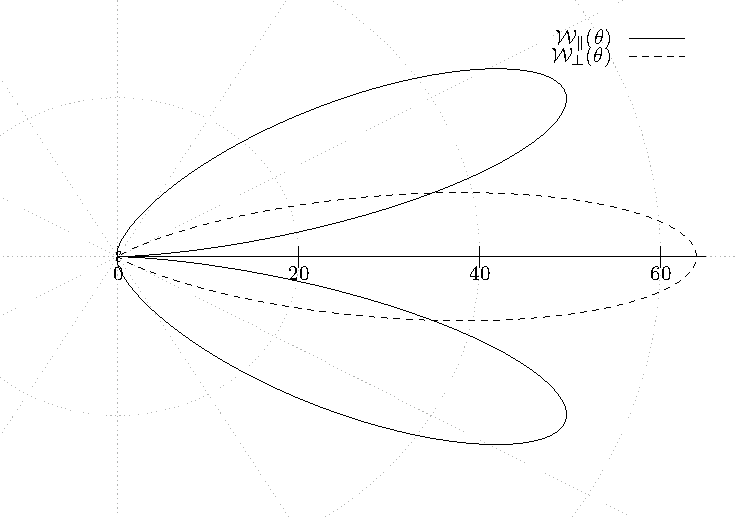
\includegraphics[width=\linewidth]{perp_par.pdf}

\begin{enumerate}
  \item $\mathcal W_\parallel = \frac{e^2}{4\pi c^2} \, w^2 \, \frac{\sin^2\theta}{(1-\beta \cos \theta)^5}$, $\theta_0 \approx \frac{1}{2 \gamma}$
  \item $\mathcal W_\perp = \frac{e^2}{4\pi c^2}  \, \frac{w^2}{(1-\beta \cos \theta)^3} 
    \left(1 - \frac{\sin^2 \theta \, \cos^2 \varphi}{\gamma^2\, (1-\beta \, \cos \theta)^2}\right)$,
    $\theta_0 = 0$, $\Delta \theta \approx 1/\gamma$
\end{enumerate}

$\gamma \gg 1 \quad I \approx I_\perp$

$\Delta t_1 \sim \frac{\rho}{c \gamma} \Rightarrow \Delta t \sim \frac{\rho}{c \gamma^3}  
\Rightarrow \omega < \omega_c = \frac{c \gamma^3}{\rho}$ 

\paragraph{Спектр и поляризация движения по окружности}
\underdev \flame

\begin{enumerate}
  \item $\v M := \sqrt{c \over 4\pi}$, $\mathcal W(\v n, t) = |\v S|\, R^2 = |\v M(t)|^2 =
    \fder{\mathcal E(t)}{t}$
  \item $\v M(\omega) = \frac{e}{c} \, \sqrt{c \over 4\pi} \intR e^{i \omega t} \,\del
    \left(\frac{\v n \times (\v n \times \v \beta)}{1 - \v n \cdot \v \beta}\right)$
  \item $t = T + R/c = t_1 - \frac 1c \v n\cdot \v x$
  \item $v M(\omega) = \frac{-i\omega e\, e^{i \omega R}}{c} \, \sqrt{c \over 4\pi} \* 
     \intR e^{i \omega (t_1 - \frac 1c \v n \cdot \v \beta)} \,
  \v n \times (\v n \times \v \beta)\, \del t_1$
  \item В поляризационном базисе и при малых углах
    $
    \begin{aligned}
      \mathcal E &= \frac{e^2 \omega^2}{4\pi^2 c}\,|-\v e_\parallel M_\parallel + \v e_\perp M_\perp|\\
      \mathcal E &= \frac{e^2}{3\pi^2 c} \*
      \left(\frac{\omega \rho}{x}\right)^2 \* \left(\frac 1{\gamma^2} + \theta^2 \right)^2\*
      \left\lvert \mathcal K_{2/3}^2 (\xi) + \tfrac{u^2}{1+u^2}\, \mathcal K_{1/3}^2 (\xi)\right\rvert\\
      u &= \gamma \theta, \quad
      x = \frac{ct}{\rho} \, \left(\tfrac{1}{\gamma^2} + \theta^2\right)^{-1/2} \;
      \xi = \frac{\omega \rho}{3c}\, \left(\tfrac{1}{\gamma^2} + \theta^2\right)^{3/2} \\
      & w_c = 3 \gamma^3 \omega_0,\quad \omega_0 = \rho/c
    \end{aligned}
    $
\end{enumerate}
возня с асимптотикой \underdev

\paragraph{Магнитотормозное излучение}
\underdev \flame

$\v E = 0 \Rightarrow \fder{\mathcal E}{t} = e \v \cdot \v E = 0$

\begin{defs}[Ларморовская частота]
\item[Ларморовская частота] $\omega_H = \frac{e H}{mc \gamma}$ 
\item[Циклотронная частота] $\frac{e H}{mc}$ 
\item[Ларморовский радиус] $\rho_H = \frac{v_\perp}{\omega_H} = \frac{v \, sin \chi}{\omega_H}$
\end{defs}

\begin{facts}
\item $w = \omega_H v\, \sin \chi $
\item $\left\{
  \begin{aligned}
    x &= x_0 + \rho_H \, \sin(\omega_H t + \alpha) \\
    y &= y_0 + \rho_H \, \cos(\omega_H t + \alpha)\\
    z &= z_0 + v\, \cos \chi t\, t
\end{aligned}\right.
  $~--- спиралька 
\item $F_\parallel= 0 \Rightarrow I = \frac{2 e^4 v^2 H^2 \sin^2 \chi}{3m^2 c^5} \propto \frac{e^4}{m^2}$
\item $\mathcal W_{\text{набл}} = \frac{1}{\sin^2 \chi} \,\mathcal W_{\text{исп}}$
\end{facts}

А что такое $W$ я не знаю. И не знаю, узнаю ли. Приятного использования.
\begin{enumerate}
  \item $\v M (t) \sum^{\infty}_{k=-\infty} \v M_k e^{-i \omega_H k t} $
  \item $W_k(\theta) = \frac{e^2k^2 \omega_H^2}{2\pi c}\,
    \Bigl\lvert\v e_\parallel \beta J_k'(k \beta \cos \theta) + i \v e_\perp \tg \theta \, J_k (k \beta \cos \theta)\Bigr\rvert^2$
  \item при $\theta = 0$ переходит в линейную, при $\theta = \pi/2$~"--- в круговую.\note{Угол между направлением и плоскостью 
    движения, так-то.}
\end{enumerate}

\plholdev{дурацкие частные случаи}

\paragraph{Рассеяние на свободных зарядах}
\end{multicols*}
\end{document}
%vim: syntax sync minlines=200
